% Packages used
\documentclass{article}
\usepackage[letterpaper, portrait, margin=2cm]{geometry}
\usepackage[utf8]{inputenc}
\usepackage[spanish, mexico]{babel}
\usepackage[T1]{fontenc}
\usepackage{float}
\usepackage{url}
\usepackage{hyperref}
\hypersetup{
    colorlinks=true,
    linkcolor=blue,
    filecolor=magenta,      
    urlcolor=cyan,
    pdftitle={Escornabot Brivoi Compactus},
    pdfpagemode=FullScreen,
}
\usepackage{array}
\usepackage{longtable}
\usepackage{multirow}
\renewcommand{\arraystretch}{1.2}
\usepackage{siunitx}
\usepackage{booktabs}
\usepackage{makecell}
\usepackage[table,xcdraw,dvipsnames]{xcolor}
\usepackage{graphicx}
\graphicspath{ {./images/Botonera/} }
\usepackage{gensymb}
\usepackage{caption}
\usepackage{subcaption}
\captionsetup[sub]{
    labelfont = bf,
    margin = 12pt,
%    indention = 18pt,
} 


%Beginning of the document
\title{Manual de Ensamble Robot Escornabot Brivoi Compactus}
\author{Wilmer Gaona Romero (@wgaonar)}
\date{Julio 2020}

\begin{document}

\maketitle

\section{Introducción}
Escornabot es un robot móvil de software y hardware abierto diseñado para la enseñanza de electrónica y programación en niños, adolescentes y no tan niños. Basado en la tarjeta Arduino Nano, destaca la sencillez de su diseño mecánico, electrónico y la estructura del código con el cual funciona. Todo esto ha sido posible por la comunidad que lo desarrolla y mantiene actualizado. Existen diversas versiones y la que corresponde a este manual es la \textbf{Brivoi Compactus} que se puede ver en la Figura \ref{fig:modelo3D}

\begin{figure}[H]
    \centering
    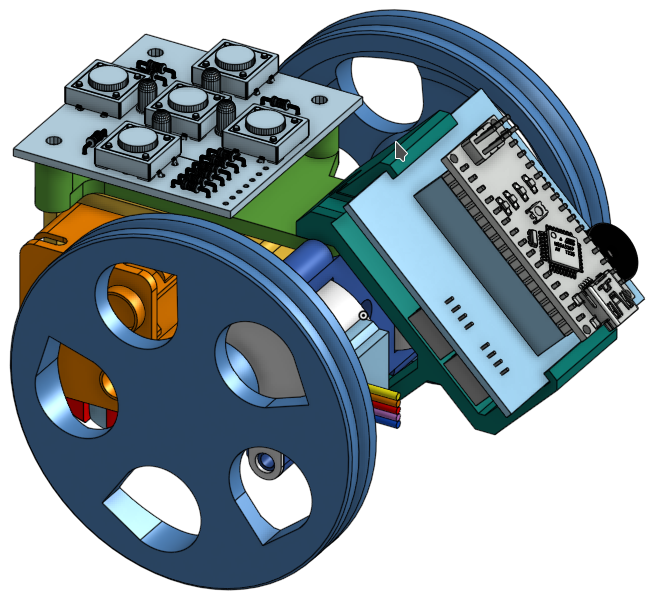
\includegraphics[width=0.6\columnwidth]{images/3DParts/portadaOnshape_1.png}
    \caption{Modelo 3D del Escornabot Brivoi Compactus}
    \label{fig:modelo3D}
\end{figure}

Esta versión cual utiliza dos tarjetas de circuitos impresos (PCB):

\begin{enumerate}
    \item Tarjeta de la botonera: \href{https://github.com/xdesig/escornabot-electronics/tree/master/Electronics/E_KEYPAD/E_KEYPAD_2.20}{E\_KeyPad V2.2 diseñada por XDeSIG}
    \item Tarjeta de control basada en el Arduino Nano:
    \href{https://github.com/xdesig/escornabot-electronics/tree/master/Electronics/EscornaCPU/1.x/1.20}{EscornaCPU V1.2 diseñada por XDeSIG}
\end{enumerate}

\section{Partes Impresas en 3D}
El cuerpo del Escornabot está compuesto por 7 partes impresas en 3D que se muestran en la Figura \ref{fig:exploded_view_1} y que se explican enseguida.

\begin{figure}[H]
    \centering
    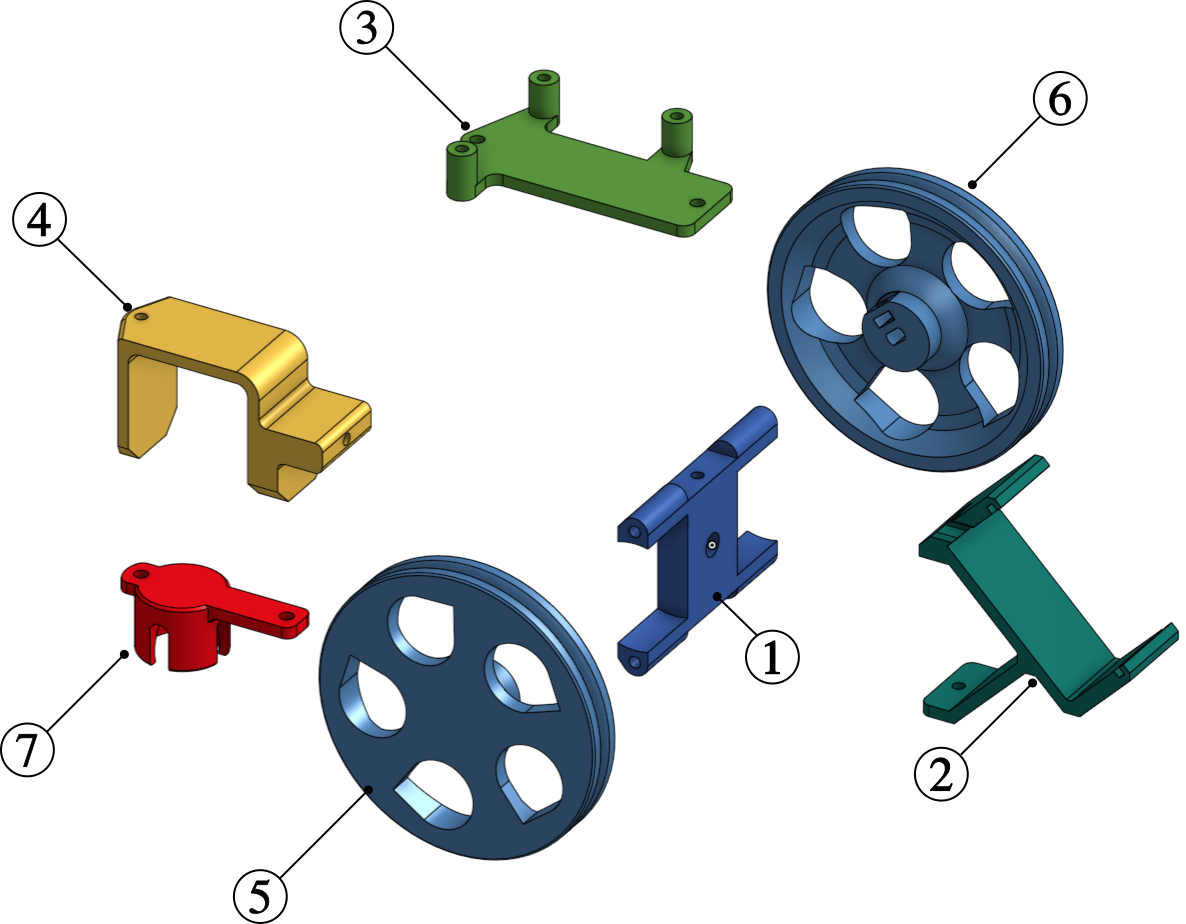
\includegraphics[width=0.8\columnwidth]{images/3DParts/Exploded_view_1.png}
    \caption{Vista Explosionada de las partes impresas en 3D}
    \label{fig:exploded_view_1}
\end{figure}

\begin{enumerate}
    \item Motor-Bracket: Parte central del robot a la que se fijan los motores y algunas de las otras piezas impresas en 3D.
    \item EscornaCPU\_1.2-Bracket: Parte a la que se fija la tarjeta de control.
    \item E-Keypad\_2.2-Bracket: Parte a la que se fija la tarjeta de la botonera.
    \item Battery-Bracket: Parte en donde van alojadas las baterías AA que alimentan el Escornabot.
    \item Wheel-Right: Rueda derecha del Escornabot.
    \item Wheel-Left: Rueda izquierda del Escornabot.
    \item Ball-Caster: Parte que aloja la esfera que sirve de pivote para que el Escornabot pueda desplazarse y girar.
\end{enumerate}

\section{Componentes Electrónicos}
\subsection{Lista de Componentes Electrónicos}
La Tabla \ref{tab:componentes_general} detalla la cantidad, descripción y la tarjeta en la que irán colocados (Botonera o la CPU) cada uno de los componentes del Escornabot. 

\begin{longtable}{|c|m{0.4\textwidth}|c|c|}
    \caption{Lista de Componentes para el Escornabot} \label{tab:componentes_general} \\ \hline 
    \multicolumn{1}{|c|}{\cellcolor[HTML]{C0C0C0}\textbf{\makecell{CANTIDAD \\ TOTAL}}} &
    \multicolumn{1}{c}{\cellcolor[HTML]{C0C0C0}\textbf{DESCRIPCIÓN}} & 
    \multicolumn{1}{|c|}{\cellcolor[HTML]{C0C0C0}\textbf{\makecell{CANTIDAD \\ BOTONERA}}} & \multicolumn{1}{c|}{\cellcolor[HTML]{C0C0C0}\textbf{\makecell{CANTIDAD \\ CPU}}} \\ \hline 
    \endfirsthead
    \caption{Lista de Componentes para el Escornabot - Continuación} \\ \hline
    \multicolumn{1}{|c|}{\cellcolor[HTML]{C0C0C0}\textbf{\makecell{CANTIDAD \\ TOTAL}}} &
    \multicolumn{1}{|c|}{\cellcolor[HTML]{C0C0C0}\textbf{DESCRIPCIÓN}} & 
    \multicolumn{1}{c|}{\cellcolor[HTML]{C0C0C0}\textbf{\makecell{CANTIDAD \\ BOTONERA}}} & \multicolumn{1}{c|}{\cellcolor[HTML]{C0C0C0}\textbf{\makecell{CANTIDAD \\ CPU}}} \\ \hline
    \endhead
    1 & Tarjeta EscornaCPU versión 1.2 & - & 1
    \\ \hline
    1 & Tarjeta E\_KeyPad versión 2.2 & 1 & -
    \\ \hline
    1 & Arduino Nano & - & 1
    \\ \hline
    2 & Motor paso a paso 28BYJ-48 & - & 2 
    \\ \hline
    1 & Driver ULN2803 & - & 1 
    \\ \hline
    1 & Zócalo de 18 pines para el driver ULN2803 & - & 1 
    \\ \hline
    1 & Portapilas para 4 pilas AA & - & -  
    \\ \hline
    1 & Terminal T-block de 5mm para alimentación & - & 1 
    \\ \hline
    4 & Resistencia 1 K$\Omega$ & 4 & - 
    \\ \hline
    9 & Resistencia 10 K$\Omega$ & 5 & 4
    \\ \hline
    1 & Resistencia 18 K$\Omega$ o de 20K$\Omega$ & - & 1 
    \\ \hline
    1 & Resistencia 22 K$\Omega$ o de 20K$\Omega$ & 1 & -
    \\ \hline
    1 & Led de 3mm Azul & 1 & - 
    \\ \hline
    1 & Led de 3mm Rojo &  1 & - 
    \\ \hline
    1 & Led de 3mm Amarillo&  1 & -
    \\ \hline
    1 & Led de 3mm Verde &  1 & -
    \\ \hline
    5 & Pulsadores de 12mm &  5 & -
    \\ \hline
    7 & Pines/headers macho a 90\degree & 7 & -
    \\ \hline
    8 & Pines/headers macho rectos  & - & 8
    \\ \hline
    1 & Puente o Jumper para pines rectos  & - & 1
    \\ \hline
    2 & Tira de 15 pines hembra que serán la base sobre la cual se colocará el Arduino Nano & - & 2 \\ \hline
    1 & Tira de 4 pines hembra si posteriormente se desea colocar un adaptador Bluetooth para conectar el Escornabot con una aplicación para teléfono móvil. & - & 1 
    \\ \hline
    1 & Interruptor de alimentación SK12F14 o SK12D07 & - & 1
    \\ \hline
    2 & Conector macho para motor paso a paso JST-XHP-5 & - & 1
    \\ \hline
    1 & Buzzer pasivo CFG12 para Arduino & - & 1
    \\ \hline
    1 & Fusible rearmable XF050 & - & 1
    \\ \hline
    1 & Diodo Schottky 1N5817 & - & 1
    \\ \hline
    2 & Condensadores cerámicos 104 de 100nF & - & 2
    \\ \hline
    6 & Cables Dupont hembra - hembra de 10cm & 6 & -
    \\ \hline
\end{longtable}

A continuación se detalla el proceso de ensamble de las partes, componentes y tarjetas de circuito impreso.

\subsection{Ensamble de la botonera E\_KeyPad V2.2}

\subsubsection{Lista de componentes de la Botonera}
La Tabla \ref{tab:componentes_botonera} muestra a detalle la cantidad de los componentes, la etiqueta en la tarjeta y la función que desempeñan.

\begin{longtable}{|c|>{\raggedright}m{0.2\textwidth}|>{\centering}m{0.15\textwidth}|m{0.45\textwidth}|}
    \caption{Descripción y funcionamiento de los componentes requeridos para la botonera} \label{tab:componentes_botonera} \\ \hline 
    \multicolumn{1}{|c|}{\cellcolor[HTML]{C0C0C0}\textbf{CANT.}} &
    \multicolumn{1}{c}{\cellcolor[HTML]{C0C0C0}\textbf{DESCRIPCIÓN}} & 
    \multicolumn{1}{|c|}{\cellcolor[HTML]{C0C0C0}\textbf{ETIQUETA}} & \multicolumn{1}{c|}{\cellcolor[HTML]{C0C0C0}\textbf{FUNCIÓN}} \\ \hline 
    \endfirsthead
    \caption{Componentes requeridos para la botonera - Continuación} \\ \hline
    \multicolumn{1}{|c|}{\cellcolor[HTML]{C0C0C0}\textbf{\makecell{CANT.}}} &
    \multicolumn{1}{c}{\cellcolor[HTML]{C0C0C0}\textbf{DESCRIPCIÓN}} & 
    \multicolumn{1}{|c|}{\cellcolor[HTML]{C0C0C0}\textbf{ETIQUETA}} & \multicolumn{1}{c|}{\cellcolor[HTML]{C0C0C0}\textbf{FUNCIÓN}} \\ \hline 
    \endhead
    4 & Resistencia 1 K$\Omega$ & R6, R8, R9, R10 & Resistencia para la activación de los Leds de la botonera.
    \\ \hline
    \multirow{7}{*}{5} & \multirow{7}{*}{Resistencia 10 K$\Omega$} & R1, R2, R3, R4  & Conforman el divisor de voltaje en conjunto con los botones para obtener diferentes valores de acuerdo al botón o switch que se ha presionado y así controlar el movimiento deseado:
    \begin{itemize}
        \item El botón S1 conectado con R1 selecciona un movimiento hacia ADELANTE.
        \item El botón S2 conectado con R2 selecciona un giro hacia la IZQUIERDA.
        \item El botón S3 conectado con R3 selecciona un movimiento hacia ATRÁS.
        \item El botón S5 conectado con R4 ejecuta la secuencia de movimientos introducida, es decir, es el botón: GO.
    \end{itemize}
    \\ \cline{3-4}
    &  & R7 & \textcolor{red}{Opcional:} Está presente en la botonera en caso de que se utilice una tarjeta de control diferente a la EscornaCPU V1.2 y en la que no se utilice la resistencia interna de PULL-UP del Arduino Nano. En el firmware del robot se tendría que definir la palabra clave: KEYBOARD\_WIRES con el valor de 3. Por precaución, esta resistencia se puede soldar.
    \\ \hline
    1 & Resistencia 22 K$\Omega$ o de 20 K$\Omega$ & R5 & La última resistencia  del divisor de voltaje: 
    \begin{itemize}
        \item El botón S4 conectado con R5 selecciona un giro hacia la DERECHA.
    \end{itemize}
    \\ \hline
    1 & Led de 3mm \textcolor{blue}{Azul} & LED1 & Led indicador de un movimiento hacia ADELANTE.
    \\ \hline
    1 & Led de 3mm \textcolor{red}{Rojo} & LED2 & Led indicador de un movimiento hacia IZQUIERDA.
    \\ \hline
    1 & Led de 3mm \textcolor{yellow}{Amarillo} & LED3 & Led indicador de un movimiento hacia ATRÁS.
    \\ \hline
    1 & Led de 3mm \textcolor{OliveGreen}{Verde} & LED4 & Led indicador de un movimiento hacia DERECHA. 
    \\ \hline
    \multirow{3}{*}{5} & \multirow{3}{*}{Pulsadores de 12mm} & S1, S2, S3, S4 & Botones para elegir los movimientos a realizar (ADELANTE, IZQUIERDA, ATRÁS Y DERECHA).
    \\ \cline{3-4}
    & & S5 & Botón GO que ejecuta la secuencia de los movimientos elegidos.
    \\ \hline 
\end{longtable}

\subsubsection{Soldadura de las Resistencias}
Las resistencias no tienen polaridad, así que no importa la orientación en que sean colocadas. Para proceder a soldarlas, colocar las resistencias teniendo presente que los valores correspondan con las etiquetas en la tarjeta. Las Figura \ref{fig:botonera_resistencias_parte2} muestra los pasos para soldar las resistencias. Tener cuidado con la ubicación de R5 para evitar confundirla con las demás ya que solo se utiliza una. (ver Figura \ref{fig:botonera_resistencias5}) .

\begin{figure}[htbp]
    \centering
    \begin{subfigure}[t]{0.3\textwidth}
        \centering
        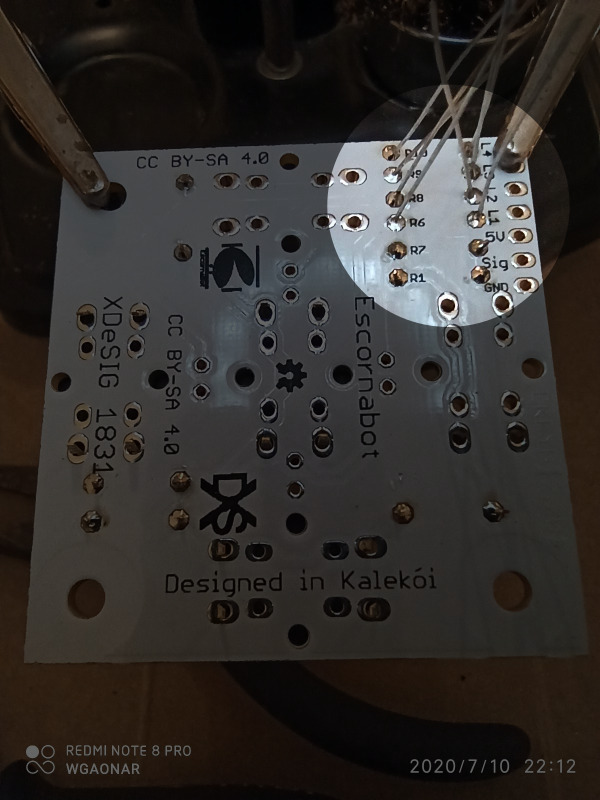
\includegraphics[width=0.9\columnwidth, height=1.2\columnwidth]{images/Botonera/botonera1.jpg}
        \caption{PCB de la botonera vista por debajo con resistencias colocadas para soldar.}
        \label{fig:botonera_resistencias1}
    \end{subfigure}%
    \begin{subfigure}[t]{0.3\textwidth}
        \centering
        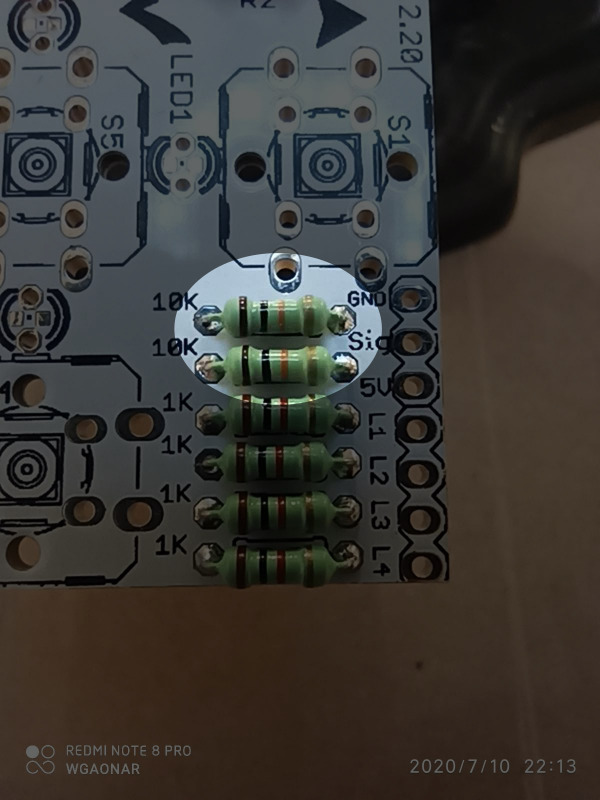
\includegraphics[width=0.9\columnwidth, height=1.2\columnwidth]{images/Botonera/botonera2.jpg}
        \caption{Soldadura R1 y R7 de 10 K$\Omega$}
        \label{fig:botonera_resistencias2}
    \end{subfigure}%
    \begin{subfigure}[t]{0.3\textwidth}
        \centering
        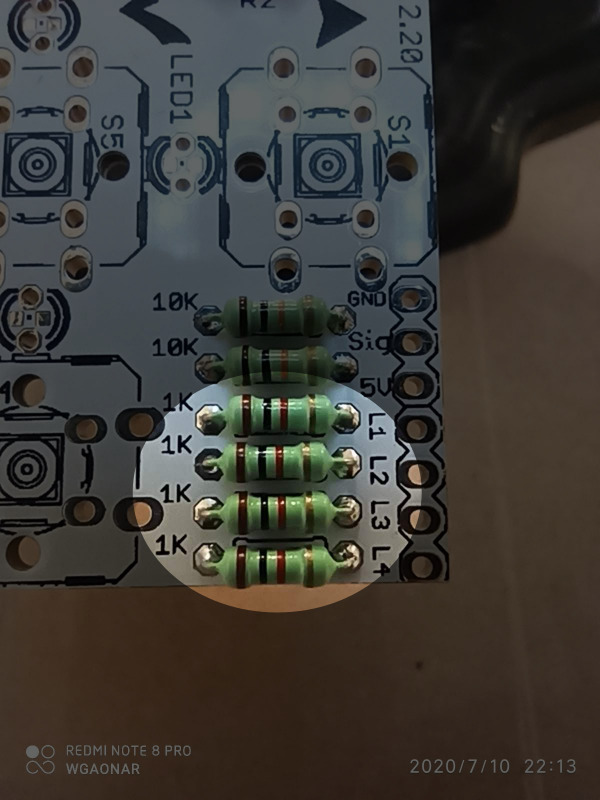
\includegraphics[width=0.9\columnwidth, height=1.2\columnwidth]{images/Botonera/botonera3.jpg}
        \caption{Soldadura de R6, R8, R9, R10 de 1 K$\Omega$}
        \label{fig:botonera_resistencias3}
     \end{subfigure}
%    \caption{Soldadura de las resistencias en la botonera parte 1.}
%    \label{fig:botonera_resistencias_parte1}
%\end{figure}

%\begin{figure}[H]
%    \ContinuedFloat \centering
    \begin{subfigure}[t]{0.3\textwidth}
        \centering
        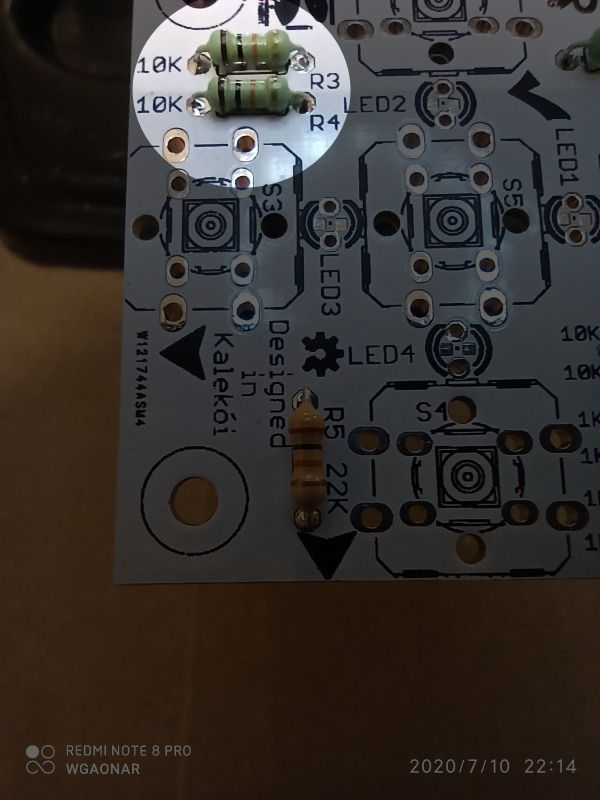
\includegraphics[width=0.9\columnwidth, height=1.2\columnwidth]{images/Botonera/botonera4.jpg}
        \caption{Soldadura de R3, R4 de 10 K$\Omega$}
        \label{fig:botonera_resistencias4}
    \end{subfigure}%
    \begin{subfigure}[t]{0.3\textwidth}
        \centering
        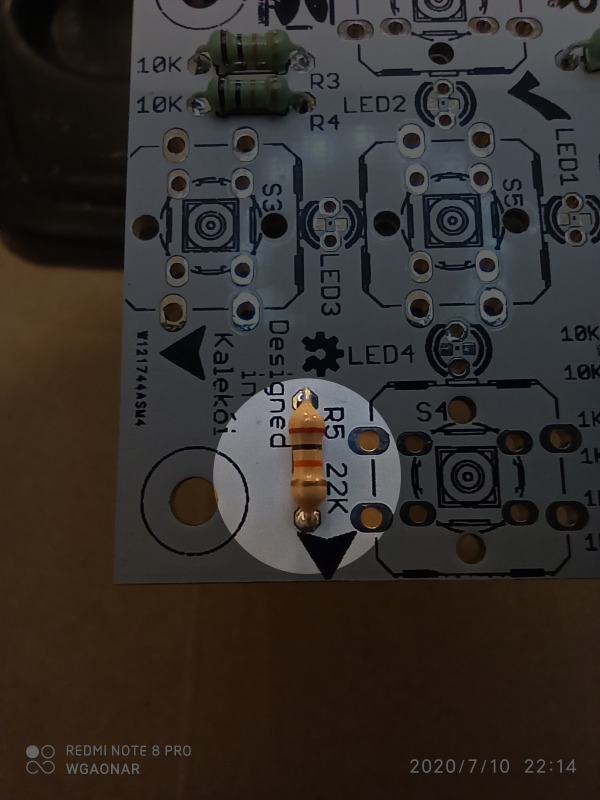
\includegraphics[width=0.9\columnwidth, height=1.2\columnwidth]{images/Botonera/botonera5.jpg}
        \caption{Soldadura de R5 de 22 K$\Omega$}
        \label{fig:botonera_resistencias5}
    \end{subfigure}%
    \begin{subfigure}[t]{0.3\textwidth}
        \centering
        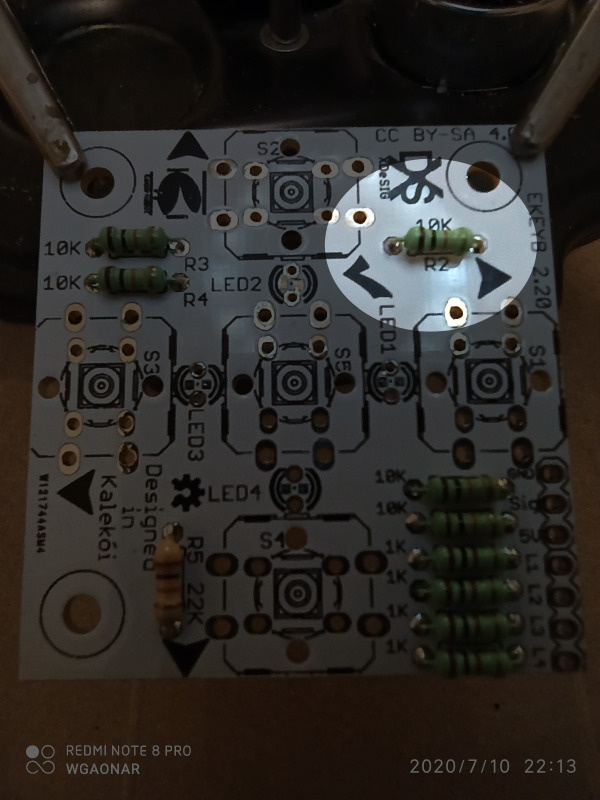
\includegraphics[width=0.9\columnwidth, height=1.2\columnwidth]{images/Botonera/botonera6.jpg}
        \caption{Soldadura de R2 de 10 K$\Omega$}
        \label{fig:botonera_resistencias6}
    \end{subfigure}
%   \caption{Soldadura de las resistencias en la botonera parte 2.}
    \caption{Soldadura de las resistencias en la botonera.}
    \label{fig:botonera_resistencias_parte2}
\end{figure}

\subsubsection{Soldadura de los Leds}
La lista de los Leds requeridos se muestra en la Tabla \ref{tab:componentes_botonera} en la que también se indica la posición de cada Led de acuerdo a su color y a su etiqueta en la tarjeta. Los Leds recomendados son de 3mm para que no estorben con los botones de 12mm. Antes de colocarlos en la tarjeta se tiene que fijar en la polaridad, ya que a diferencia de las resistencias, \textbf{\textcolor{red}{los Leds si tienen polaridad}}. Para ello, en la base cilíndrica del cuerpo de cristal del Led se puede observar una parte plana justo donde se conecta la terminal más corta que es la posición del cátodo o la terminal negativa del Led. 

\begin{figure}[H]
    \centering
    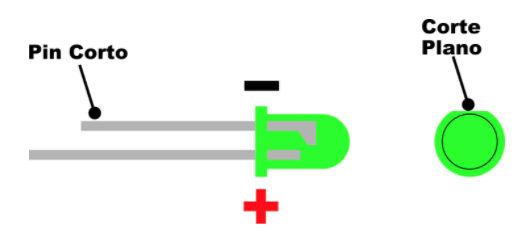
\includegraphics[width=0.5\columnwidth]{images/Botonera/led0}
    \caption{Esquema de polaridad del led.}
    \label{fig:poladirad_led}
\end{figure}

Si se observa la tarjeta de frente, el cátado de cada uno de los leds se orienta a la izquierda. Además, en el dibujo indicador de la tarjeta se puede observar, aunque muy sutilmente, esta parte plana. Soldar cada Led fijándose que la polaridad y el color coincida con la etiqueta en la tarjeta. Al finalizar de soldar todos los Leds, recortar los sobrantes. Los pasos en la soldadura de los Leds se puede observar en la Figura \ref{fig:botonera_leds}.

\begin{figure}[H]
    \centering
    \begin{subfigure}[t]{0.3\textwidth}
        \centering
        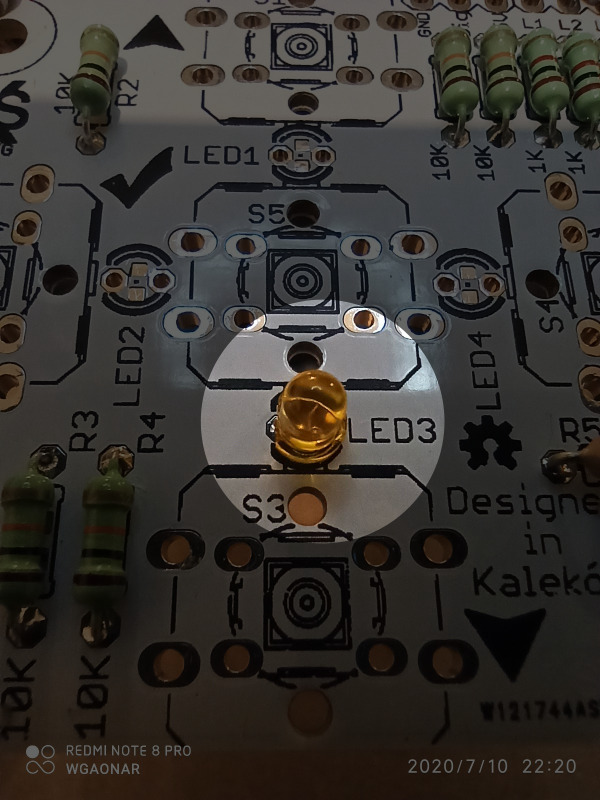
\includegraphics[width=0.9\columnwidth, height=1.2\columnwidth]{images/Botonera/led1.jpg}
        \caption{Led 3: \textcolor{yellow}{Amarillo}.}
        \label{fig:botonera_led1}
    \end{subfigure}%
    \begin{subfigure}[t]{0.3\textwidth}
        \centering
        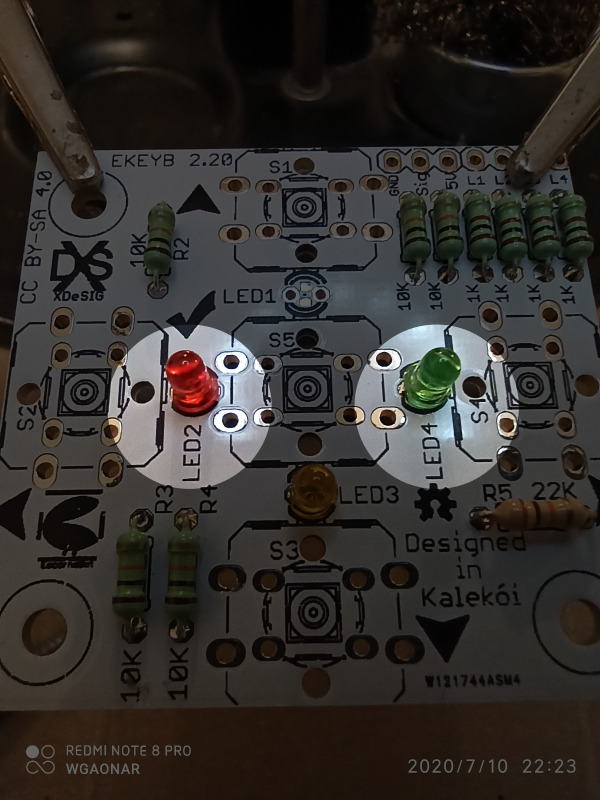
\includegraphics[width=0.9\columnwidth, height=1.2\columnwidth]{images/Botonera/led2.jpg}
        \caption{Led 2: \textcolor{red}{Red} y Led 4: \textcolor{OliveGreen}{Verde}.}
        \label{fig:botonera_led2}
    \end{subfigure}%
    \begin{subfigure}[t]{0.3\textwidth}
        \centering
        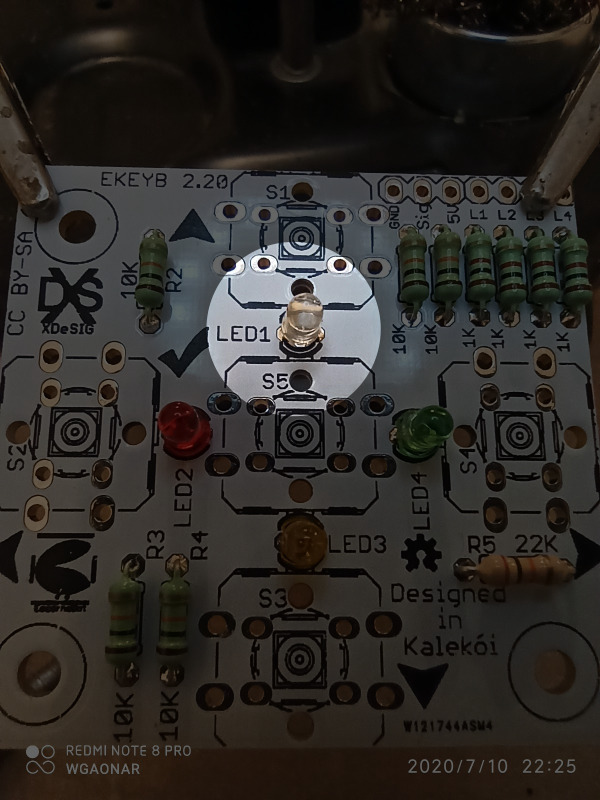
\includegraphics[width=0.9\columnwidth, height=1.2\columnwidth]{images/Botonera/led3.jpg}
        \caption{Led 1: \textcolor{blue}{Azul}. (Aunque el cuerpo es transparente)}
        \label{fig:botonera_led3}
    \end{subfigure}
    
%    \vspace{0.5cm}
%    \begin{subfigure}[t]{0.3\textwidth}
%        \centering
%        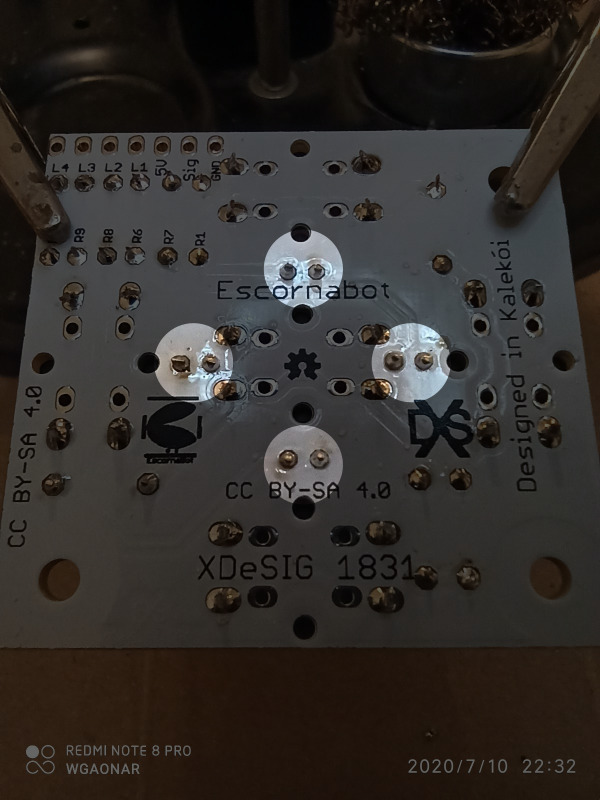
\includegraphics[width=0.9\columnwidth, height=1.2\columnwidth]{images/Botonera/led4.jpg}
%        \caption{Terminales de los Leds recortadas.}
%        \label{fig:botonera_led4}
%    \end{subfigure}
    \caption{Soldadura de los leds en la botonera.}
    \label{fig:botonera_leds}
\end{figure}

\subsubsection{Soldadura de los Botones}
La soldadura de los botones se puede observar en la Figura \ref{fig:botones_soldadura}. Es simple de realizar ya que tienen las terminales dobladas formando un resorte para que se queden fijas en la tarjeta, basta insertarlos con cierta fuerza hasta que se escuche el sonido de un “click”, el cual indica que están fijos en su posición. 

\begin{figure}[H]
    \centering
    \begin{subfigure}[t]{0.3\textwidth}
        \centering
        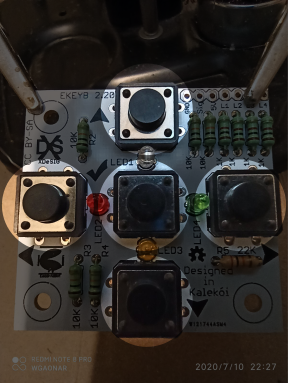
\includegraphics[width=0.9\columnwidth, height=1.2\columnwidth]{images/Botonera/botones1.png}
        \caption{Botones Soldados}
        \label{fig:botones_frente}
    \end{subfigure}%
    \begin{subfigure}[t]{0.3\textwidth}
        \centering
        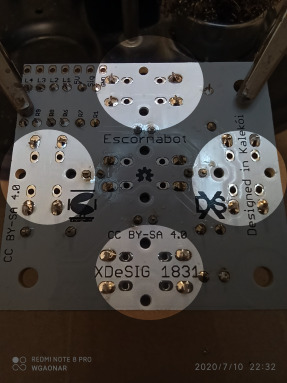
\includegraphics[width=0.9\columnwidth, height=1.2\columnwidth]{images/Botonera/botones2.jpg}
        \caption{Vista posterior con las terminales de los botones.}
        \label{fig:botones_posterior}
    \end{subfigure}
    \caption{Soldadura de los botones}
    \label{fig:botones_soldadura}
\end{figure}

\subsubsection{Soldadura de los Pines de Conexión}
La conexión con la placa EscornaCPU que contiene al Arduino Nano se realiza a través de 6 o 7 pines con las funciones listadas en la Tabla \ref{tab:pines_de_conexión}. La soldadura de los pines tipo macho a 90\degree se pueden ver en la Figura \ref{fig:pines_de_conexión}.

\begin{longtable}{|c|c|m{0.6\textwidth}|}
    \caption{Identificación de los pines de conexión \\ entre la botonera y la tarjeta EscornaCPU (Arduino Nano)} \label{tab:pines_de_conexión} \\ \hline 
    \multicolumn{1}{|c|}{\cellcolor[HTML]{C0C0C0}\textbf{PIN}} &
    \multicolumn{1}{|c|}{\cellcolor[HTML]{C0C0C0}\textbf{ETIQUETA}} & \multicolumn{1}{c|}{\cellcolor[HTML]{C0C0C0}\textbf{FUNCIÓN}} \\ \hline 
    \endfirsthead
    \caption{Identificación de los pines de conexión entre la botonera y la tarjeta EscornaCPU (Arduino Nano) - Continuación} \\ \hline
    \multicolumn{1}{|c|}{\cellcolor[HTML]{C0C0C0}\textbf{PIN}} &
    \multicolumn{1}{|c|}{\cellcolor[HTML]{C0C0C0}\textbf{ETIQUETA}} & \multicolumn{1}{c|}{\cellcolor[HTML]{C0C0C0}\textbf{FUNCIÓN}} \\ \hline 
    \endhead
    1 & GND & Trae la señal de tierra (0V) desde la tarjeta EscornaCPU (Arduino Nano). 
    \\ \hline
    2 & Signal & Lleva la señal analógica del voltaje resultante al presionar uno de los botones.
    \\ \hline
    3 & 5V & \textcolor{red}{Opcional:} Está presente en la botonera en caso de que se utilice una tarjeta de control diferente a la EscornaCPU versión 1.2 y en la que no se utilice la resistencia interna de PULL-UP del Arduino Nano. En el firmware del robot se tendría que definir la palabra clave: KEYBOARD\_WIRES con valor de 3.
    \\ \hline
    4 & L1 & Señal de control para el Led 1 de color \textcolor{blue}{azul} que indica un movimiento hacia ADELANTE.
    \\ \hline
    5 & L2 & Señal de control para el Led 2 de color \textcolor{red}{rojo} que indica un movimiento hacia IZQUIERDA. 
    \\ \hline
    6 & L3 & Señal de control para el Led 3 de color \textcolor{yellow}{amarillo} que indica un movimiento hacia ATRÁS. 
    \\ \hline
    7 & L4 & Señal de control para el Led 4 de color \textcolor{OliveGreen}{verde} que indica un movimiento hacia DERECHA.
    \\ \hline
\end{longtable}

\begin{figure}[H]
    \centering
    \begin{subfigure}[t]{0.3\textwidth}
        \centering
        \includegraphics[width=0.9\columnwidth, height=1.2\columnwidth]{images/Botonera/pinesdeConexión1.png}
        \caption{Pines de conexión vistos por detrás.}
        \label{fig:pines_de_conexión1}
    \end{subfigure}%
    \begin{subfigure}[t]{0.3\textwidth}
        \centering
        \includegraphics[width=0.9\columnwidth, height=1.2\columnwidth]{images/Botonera/pinesdeConexión2.png}
        \caption{Pines de conexión vistos de frente.}
        \label{fig:pines_de_conexión2}
    \end{subfigure}
    \caption{Soldadura de los pines de conexión en la botonera.}
    \label{fig:pines_de_conexión}
\end{figure}

\subsubsection{Prueba de la botonera terminada}
La prueba de la tarjeta de la botonera consiste en probar el funcionamiento de los Leds y de los Botones. Para probar el funcionamiento de los Leds basta con energizar o conectar cada Led a 0 y 5V. Para esto, se puede traer el Voltaje desde los pines GND y 5V del Arduino Nano través de dos cables conectados a los pines GND y L1/L2/L3/L4 que alimentan a cada Led en la Botonera. Como ejemplo, se puede observar en la Figura \ref{fig:botonera_PruebaLeds} como al conectar uno de los cables al pin GND y el otro cable a cualquiera de los pines L1/L2/L3/L4 se enciende el Led correspondiente. En caso de que no encendieran verificar la orientación (polaridad) de los Leds en la botonera y el valor de las resistencias que debe ser de 1 K$\Omega$.

\begin{figure}[H]
    \centering
    \begin{subfigure}[t]{0.3\textwidth}
        \centering
        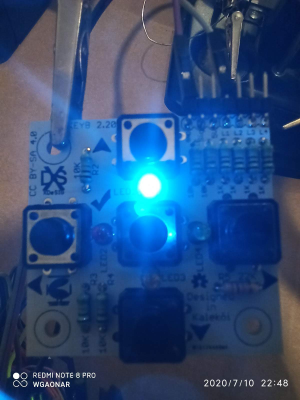
\includegraphics[width=0.9\columnwidth, height=1.2\columnwidth]{images/Botonera/botonera_ensambleLed_1.png}
        \caption{Prueba del Led 1 de color \textcolor{blue}{azul} conectacto al pin L1.}
        \label{fig:botonera_ensambleLed_1}
    \end{subfigure}%
    \begin{subfigure}[t]{0.3\textwidth}
        \centering
        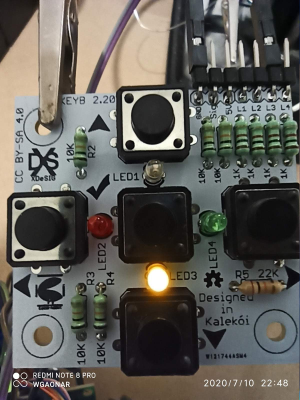
\includegraphics[width=0.9\columnwidth, height=1.2\columnwidth]{images/Botonera/botonera_ensambleLed_3.png}
        \caption{Prueba del Led 3 de color \textcolor{yellow}{amarillo} conectado al pin L3.}
        \label{fig:botonera_ensambleLed_3}
    \end{subfigure}%
    \begin{subfigure}[t]{0.3\textwidth}
        \centering
        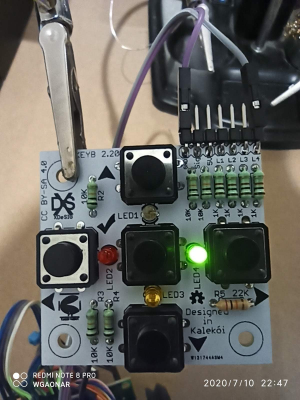
\includegraphics[width=0.9\columnwidth, height=1.2\columnwidth]{images/Botonera/botonera_ensambleLed_4.png}
        \caption{Prueba del Led 4 de color \textcolor{OliveGreen}{verde} conectado al pin L4.}
        \label{fig:botonera_ensambleLed_4}
    \end{subfigure}
    \caption{Soldadura de los pines de conexión en la botonera.}
    \label{fig:botonera_PruebaLeds}
\end{figure}

Por otro lado, para probar el funcionamiento de los botones se necesita de un multímetro con el objetivo de medir el valor de la resistencia al accionar cualquiera de los botones. Para esto seguir el siguiente procedimiento:
\begin{enumerate}
    \item Colocar el multímetro en la escala de 200 K$\Omega$.
    \item Conectar la punta de prueba negra en el pin de la botonera con la etiqueta: \textbf{GND}.
    \item Conectar la punta de prueba \textcolor{red}{roja} en el pin de la botonera con la etiqueta: \textbf{Sig}.
    \item Pulsar cada uno de los botones y comparar el valor de la resistencia indicada por el multímetro con los siguientes valores:
    \begin{itemize}
        \item Al pulsar el botón ubicado encima del Led 1 de color  \textcolor{blue}{azul}, el multímetro indicará 10 K$\Omega$ aproximadamente.
        \item Al pulsar el botón ubicado a la izquierda del Led 2 de color  \textcolor{red}{rojo}, el multímetro indicará 20 K$\Omega$ aproximadamente.
        \item Al pulsar el botón ubicado abajo del Led 3 de color  \textcolor{yellow}{amarillo}, el multímetro indicará 30 K$\Omega$ aproximadamente.
        \item Al pulsar el botón ubicado a la derecha del Led 4 de color \textcolor{OliveGreen}{verde}, el multímetro indicará 62 K$\Omega$ aproximadamente.
        \item Al pulsar el botón del centro, el multímetro indicará 40 K$\Omega$ aproximadamente.
    \end{itemize}
\end{enumerate}

El funcionamiento de la botonera se basa en un divisor de voltaje, el cual, al pulsar cada uno de los botones varía el voltaje en un rango de 0-5V. Esta señal de voltaje es la que va conectadad al pin con la etiqueta \textbf{Sig} de la botonera. El esquema eléctrico de la botonera, así como un esquema simplificado y las ecuaciones del funcionamiento del circuito divisor de voltaje se muestran en la Figura \ref{fig:botonera_divisor_voltaje_1}.

\begin{figure}[H]
    \centering
    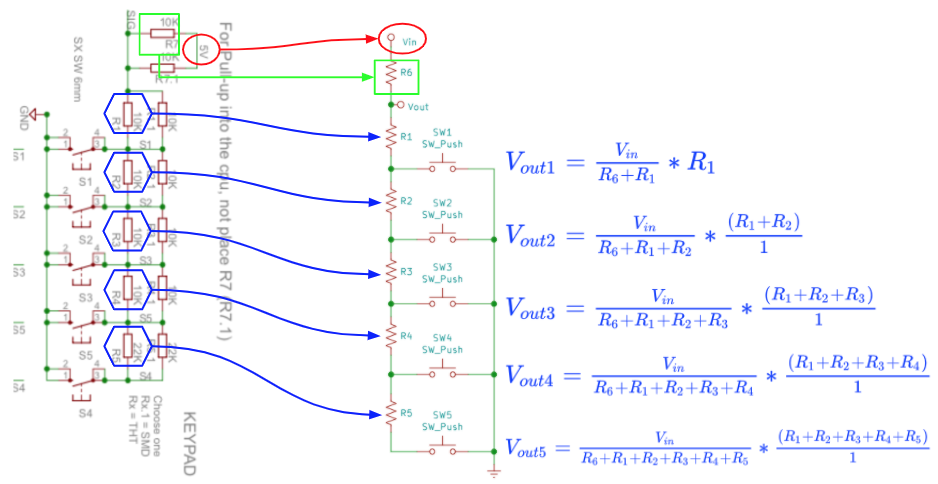
\includegraphics[width=0.9\columnwidth]
    {images/Botonera/botonera_divisor_voltaje.png}
    \caption{Esquemas y ecuaciones del circuito divisor de voltaje que conforma la botonera}
    \label{fig:botonera_divisor_voltaje_1}
\end{figure}

\subsection{Ensamble de la tarjeta de control EscornaCPU V1.2}
\subsubsection{Lista de componentes de la tarjeta de control}
\begin{longtable}{|c|>{\raggedright}m{0.17\textwidth}|>{\centering}m{0.15\textwidth}|m{0.5\textwidth}|}
    \caption{Descripción y funcionamiento de los componentes requeridos para la tarjeta de control} \label{tab:componentes_tarjeta_de_control} \\ \hline 
    \multicolumn{1}{|c|}{\cellcolor[HTML]{C0C0C0}\textbf{CANT.}} &
    \multicolumn{1}{c}{\cellcolor[HTML]{C0C0C0}\textbf{DESCRIPCIÓN}} & 
    \multicolumn{1}{|c|}{\cellcolor[HTML]{C0C0C0}\textbf{ETIQUETA}} & \multicolumn{1}{c|}{\cellcolor[HTML]{C0C0C0}\textbf{FUNCIÓN}} \\ \hline 
    \endfirsthead
    \caption{Descripción y funcionamiento de los componentes requeridos para la tarjeta de control - Continuación} \\ \hline
    \multicolumn{1}{|c|}{\cellcolor[HTML]{C0C0C0}\textbf{\makecell{CANT.}}} &
    \multicolumn{1}{c}{\cellcolor[HTML]{C0C0C0}\textbf{DESCRIPCIÓN}} & 
    \multicolumn{1}{|c|}{\cellcolor[HTML]{C0C0C0}\textbf{ETIQUETA}} & \multicolumn{1}{c|}{\cellcolor[HTML]{C0C0C0}\textbf{FUNCIÓN}} \\ \hline 
    \endhead
    1 & Arduino Nano & Arduino Nano & Tarjeta de desarrollo y programación basada en el microcontrolador ATmega328 
    \\ \hline
    1 & Driver ULN2803 & IC1 ULN2803 & Circuito integrado que es el enlace o interfaz entre las señales de control provenientes del Arduino Nano y los motores paso a paso 28BYJ-48. \newline \textbf{Nota:} \textcolor{red}{Este circuito no se solda}, se coloca sobre un zócalo o base que si irá soldado a la tarjeta. 
    \\ \hline
    1 & Zócalo de 18 pines & IC1 ULN2803 & Base que soldada a la tarjeta sobre la que se coloca el driver ULN2803. 
    \\ \hline
    1 & Terminal T-block (3.5mm o 5mm)  & GND $+$ & Terminal de tornillos a los que se conectarán los cables provenientes del portapilas que alimentará la tarjeta de control y los motores paso a paso. 
    \\ \hline
    \multirow{8}{*}{4} & \multirow{8}{0.15\textwidth}{Resistencia 10 K$\Omega$} & R1 & \textcolor{red}{Opcional:} Está presente en la tarjeta de control en caso de que se utilice una botonera diferente a la E\_KeyPad V2.2 que no cuente con esta resistencia y que no se utilice la resistencia interna de PULL\_UP del Arduino Nano. En el firmware del robot se tendría que definir la palabra clave: KEYBOARD\_WIRES con el valor de 3. Por precaución, esta resistencia se puede soldar. 
    \\ \cline{3-4}
    &  & R2 & La primera resistencia del divisor de voltaje que reduce el voltaje de 5.0V a 3.3V que va desde el pin 1 del Arduino hacia el pin de transmisión del adaptador Bluetooth, en caso de que se desea conectar y utilizar. 
    \\ \cline{3-4}
    &  & R4, R5 & \textcolor{red}{Opcionales:} Están presentes en la tarjeta de control en caso de que se desea conectar el Escornabot a una red WiFi a través de un módulo un ESP-01.  
    \\ \hline
    1 & Resistencia 18 K$\Omega$ o 20 K$\Omega$ & R3 & La segunda resistencia del divisor de voltaje que reduce el voltaje de 5.0V a 3.3V que va desde el pin 1 del Arduino hacia el pin de transmisión del adaptador Bluetooth, en caso de que se desea conectar y utilizar. 
    \\ \hline
    \multirow{4}{*}{8} & \multirow{4}{0.15\textwidth}{Pines / headers macho rectos} & A0, A1, A2, A3, A7, GND & 6 Pines de conexión con la tarjeta de la botonera. \\ \cline{3-4}
    & & BUZZ ON & 2 Pines que permitirán activar / desactivar de forma manual el buzzer del Escornabot a través de la colocación de un puente o Jumper para pines rectos.
    \\ \hline
    2 & Tira de 15 pines hembra & D12 & Base soldada sobre la cual se colocará el Arduino Nano
    \\ \hline
    1 & Tira de 4 pines hembra & BlueT & \textcolor{red}{Opcional:} En caso de que se desee colocar un adaptador Bluetooth para conectar el Escornabot con una aplicación para teléfono móvil.
    \\ \hline
    1 & Interruptor de alimentación SK12F14 o SK12D07 & S7 & Interruptor general que enciende o apaga el Escornabot.
    \\ \hline
    1 & Buzzer pasivo CFG12 para Arduino & Z1 & Emitir un sonido frente a cada movimiento o instrucción ejecutada por el Escornabot.
    \\ \hline
    1 & Fusible Rearmable XF050 & F1 & Interruptor de seguridad que se abre frente al paso de una cantidad de corriente que podría quemar el Arduino Nano u otro componente de la tarjeta de control.
    \\ \hline
    1 & Diodo Schottky 1N5817 & D1 & Diodo utilizado para la protección del circuito frente a polaridad invertida.
    \\ \hline
    2 & Condensadores cerámicos 104 de 100nF & C1, C3 & Eliminación de ruido eléctrico en la señal de alimentación de la Tarjeta y en el Driver ULN2803.
    \\ \hline
\end{longtable}

\subsubsection{Soldadura de las Resistencias}
Soldar las resistencias de forma similar a la Botonera. Teniendo cuidado de no confundir los valores. La Figura \ref{fig:cpu_resistencias} muestra el soldado de cada una de las resistencias.

\begin{figure}[H]
    \centering
    \begin{subfigure}[t]{0.3\textwidth}
        \centering
        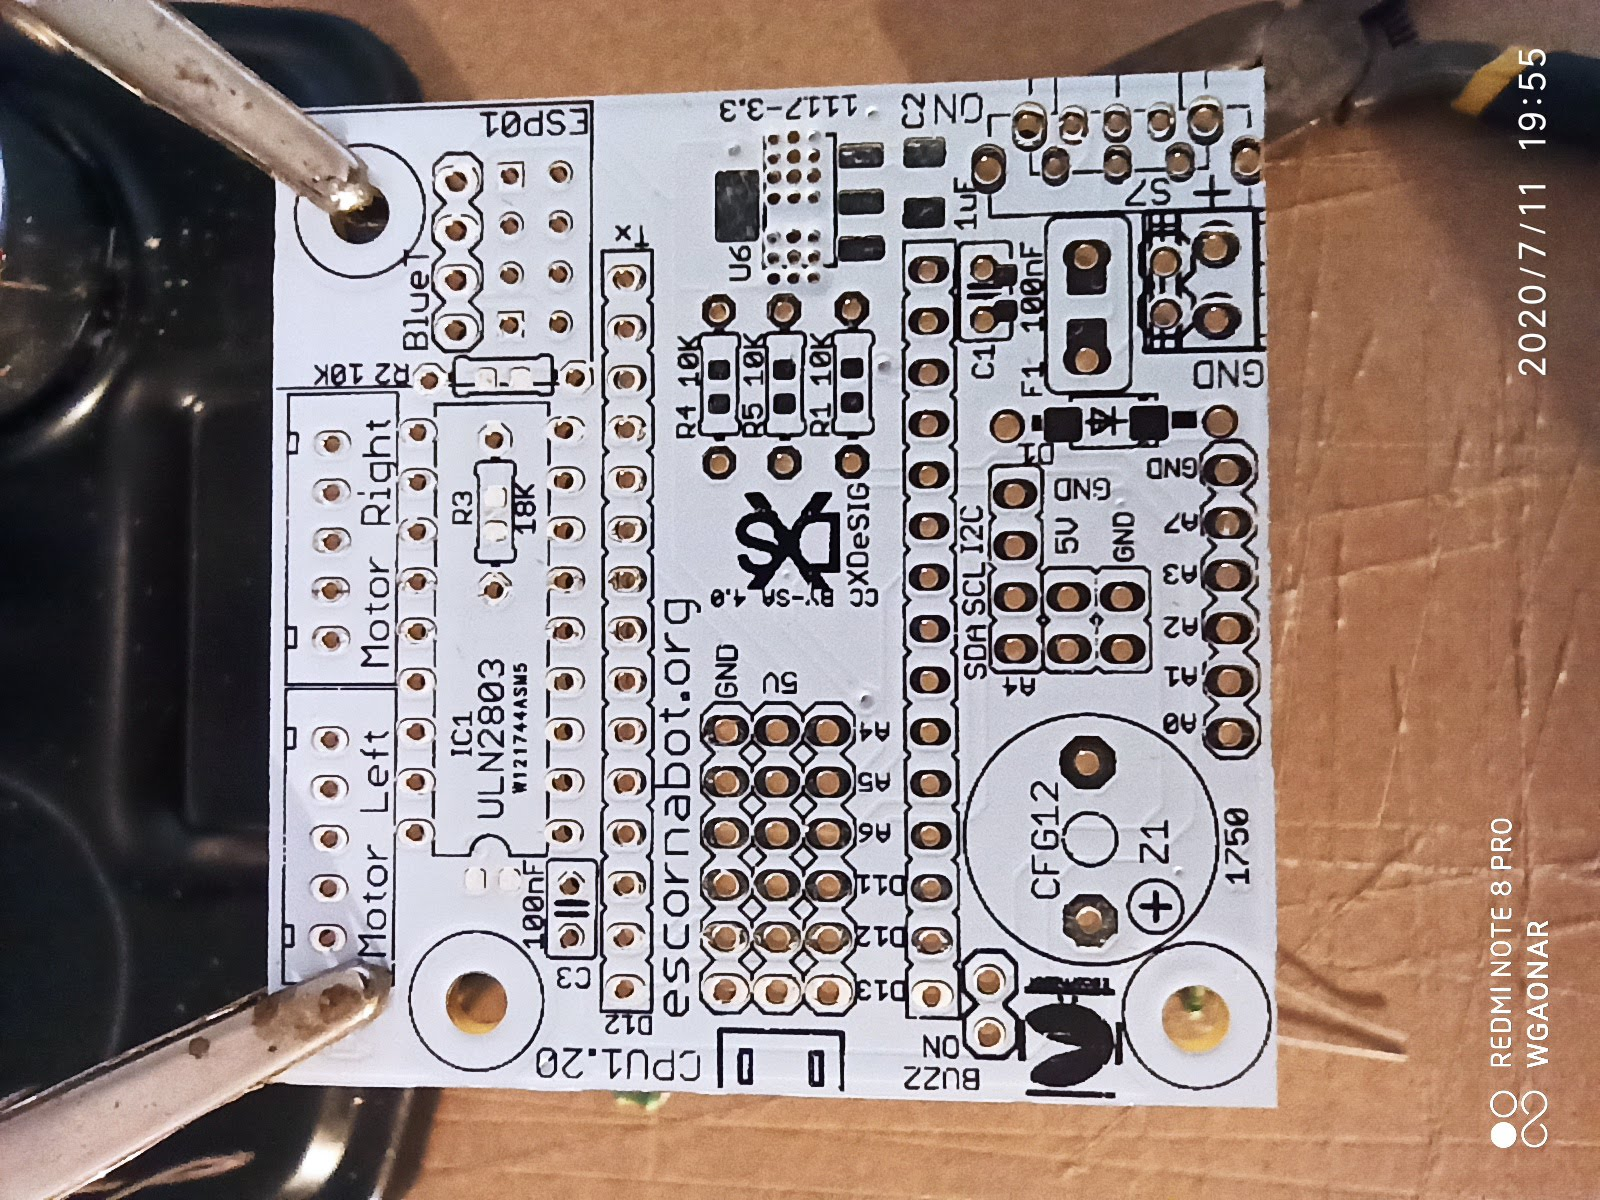
\includegraphics[width=0.9\columnwidth, height=1.2\columnwidth]{images/CPU/cpu_inicial.jpg}
        \caption{Tarjeta de control}
        \label{fig:cpu_inicial}
    \end{subfigure}%
    \begin{subfigure}[t]{0.3\textwidth}
        \centering
        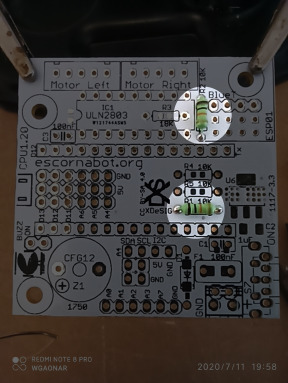
\includegraphics[width=0.9\columnwidth, height=1.2\columnwidth]{images/CPU/cpu_resistencias_1.jpg}
        \caption{Soldadura de R1 y R2 de 10 K$\Omega$ .}
        \label{fig:cpu_resistencias_1}
    \end{subfigure}%
    \begin{subfigure}[t]{0.3\textwidth}
        \centering
        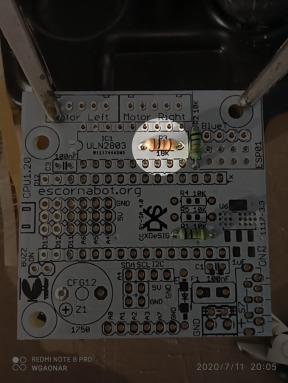
\includegraphics[width=0.9\columnwidth, height=1.2\columnwidth]{images/CPU/cpu_resistencias_2.jpg}
        \caption{Soldadura de R3 de 18 K$\Omega$.}
        \label{fig:cpu_resistencias_2}
    \end{subfigure}
    \caption{Soldadura de los resistencias en la tarjeta de control}
    \label{fig:cpu_resistencias}
\end{figure}

\subsubsection{Soldadura del diodo y los condensadores}
Antes de soldar el \textbf{diodo} se debe observar su polaridad, ya que este elemento permite el paso de la corriente en una única dirección, por lo que es importante que quede soldado de la manera correcta. El esquema con el que se representa a este componente consiste en un triángulo con una barra horizontal en uno de sus vértices. La dirección del triángulo indica la dirección de la corriente, mientras que la barra horizontal indica el \textbf{no} paso de la corriente. Este esquema se encuentra dibujado en la tarjeta para orientar al diodo de forma correcta. Por otro lado, en el componente únicamente se señala la barra horizontal de color gris, suficiente para orientarlo en la tarjeta tal como se muestra en la Figura \ref{fig:cpu_diodo_1}.

Por otro lado, los condensadores cerámicos son elementos que \textbf{no} tienen polaridad, a diferencia de los electrolíticos que sí la tienen. En este caso los condensadores 104 se pueden soldar sin importar la orientación en que se coloquen. Las Figuras \ref{fig:cpu_codensadores_1} y \ref{fig:cpu_condensadores_2} muestran la soldadura de estos dos condensadores y el aspecto de la tarjeta de control.

\begin{figure}[H]
    \centering
    \begin{subfigure}[t]{0.3\textwidth}
        \centering
        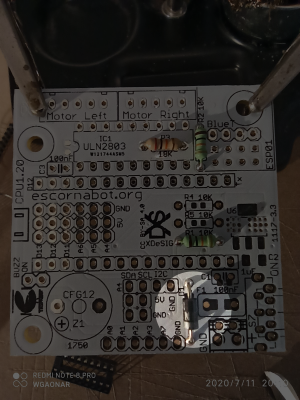
\includegraphics[width=0.9\columnwidth, height=1.2\columnwidth]{images/CPU/cpu_diodo_1.png}
        \caption{Soldadura del diodo Schottky 1N5817}
        \label{fig:cpu_diodo_1}
    \end{subfigure}%
    \begin{subfigure}[t]{0.3\textwidth}
        \centering
        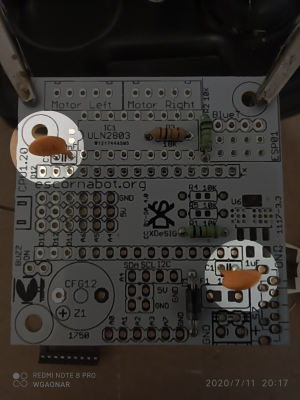
\includegraphics[width=0.9\columnwidth, height=1.2\columnwidth]{images/CPU/cpu_condensadores_1.png}
        \caption{Soldadura de los condensadores cerámicos 104 de 100nF.}
        \label{fig:cpu_codensadores_1}
    \end{subfigure}%
    \begin{subfigure}[t]{0.3\textwidth}
        \centering
        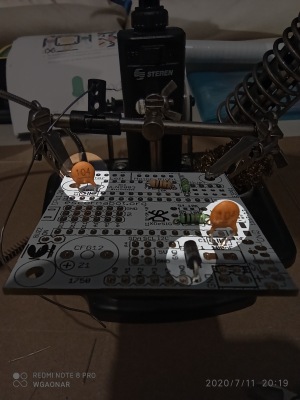
\includegraphics[width=0.9\columnwidth, height=1.2\columnwidth]{images/CPU/cpu_condensadores_2.png}
        \caption{Vista inclinada de la tarjeta de control}
        \label{fig:cpu_condensadores_2}
    \end{subfigure}
    \caption{Soldadura del diodo Schottky 1N5817 y los condensadores cerámicos 104 de 100nF en la tarjeta de control.}
    \label{fig:cpu_diodo_condensadores}
\end{figure}

\subsubsection{Soldadura del Zócalo de 18 Pines}
El zócalo de 18 pines se utiliza para colocar encima el driver ULN2803, ya que no es recomendable soldarlo de forma directa a la placa debido a que se puede quemar por el calor aplicado y además, en caso de que se necesite reemplazar a futuro, pueda realizarse sin tener que desoldarlo de la tarjeta. Para soldarlo hay que tener presente que sí tiene una orientación específica con la muesca que tiene en uno de sus extremos orientada hacia la izquierda, tal como se muestra en la Figura \ref{fig:cpu_zocalo_1} teniendo cuidado de acomodarlo de forma correcta para que la resistencia R3 de 18 K$\Omega$ no le estorbe ya que esta última queda debajo y oculta por el zócalo. Como recomendación para una adecuada soldadura, se pueden soldar únicamente dos terminales del zócalo y acomodarlo de forma tal que no quede levantado antes de soldar las terminales restantes, como se puede observar en las Figuras \ref{fig:cpu_zocalo_2} y  \ref{fig:cpu_zocalo_3} respectivamente.

\begin{figure}[H]
    \centering
    \begin{subfigure}[t]{0.3\textwidth}
        \centering
        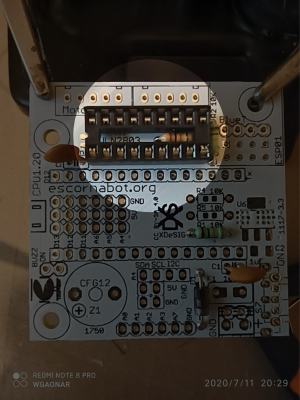
\includegraphics[width=0.9\columnwidth, height=1.2\columnwidth]{images/CPU/cpu_zocalo_1.png}
        \caption{Soldadura del diodo Schottky 1N5817}
        \label{fig:cpu_zocalo_1}
    \end{subfigure}%
    \begin{subfigure}[t]{0.3\textwidth}
        \centering
        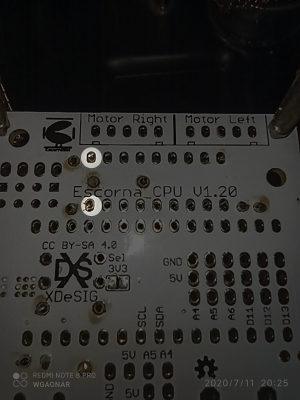
\includegraphics[width=0.9\columnwidth, height=1.2\columnwidth]{images/CPU/cpu_zocalo_2.png}
        \caption{Soldadura de los condensadores cerámicos 104 de 100nF.}
        \label{fig:cpu_zocalo_2}
    \end{subfigure}%
    \begin{subfigure}[t]{0.3\textwidth}
        \centering
        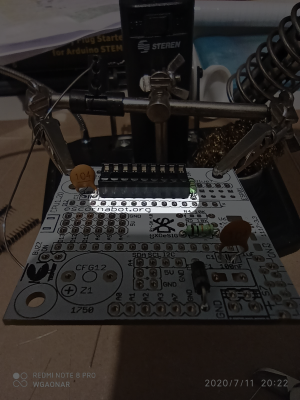
\includegraphics[width=0.9\columnwidth, height=1.2\columnwidth]{images/CPU/cpu_zocalo_3.png}
        \caption{Vista inclinada de la tarjeta de control}
        \label{fig:cpu_zocalo_3}
    \end{subfigure}
    \caption{Soldadura del zócalo de 18 pines en la tarjeta de control.}
    \label{fig:cpu_zocalo}
\end{figure}

\subsubsection{Soldadura del Buzzer, sus Pines de Activación y los Pines de Conexión a la Botonera}
Proceder a soldar 2 pines / headers rectos tal como se muestra en la Figura \ref{fig:cpu_pines_buzzer_1} los cuales permitirán activar / desactivar el buzzer de forma manual a través de la colocación de un puente o jumper.

En segundo lugar, colocar el buzzer fijándose en la etiqueta: $\oplus$ que tiene estampada en la parte superior para que coincida con la misma marca impresa en la tarjeta. Una vez realizado esto, soldar el buzzer para obtener el resultado que se muestra en la Figura \ref{fig:cpu_buzzer_1}.

En tercer lugar, soldar 6 pines / headers rectos para conectar los cables que provienen de la botonera. \textbf{Nota:} es muy importante fijarse en la orientación para que queden hacia abajo, como se puede ver en la Figura \ref{fig:cpu_pines_botonera_1}.

\begin{figure}[H]
    \centering
    \begin{subfigure}[t]{0.3\textwidth}
        \centering
        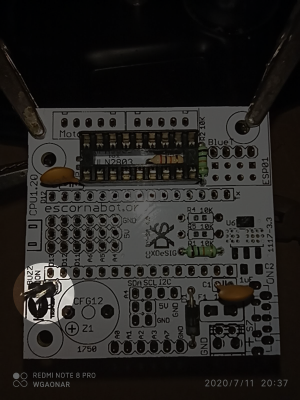
\includegraphics[width=0.9\columnwidth, height=1.2\columnwidth]{images/CPU/cpu_postes_buzzer_1.png}
        \caption{Soldadura de los pines para la activación / desactivación del buzzer.}
        \label{fig:cpu_pines_buzzer_1}
    \end{subfigure}%
    \begin{subfigure}[t]{0.3\textwidth}
        \centering
        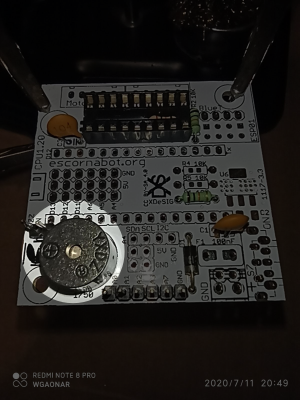
\includegraphics[width=0.9\columnwidth, height=1.2\columnwidth]{images/CPU/cpu_buzzer_1.png}
        \caption{Soldadura del buzzer}
        \label{fig:cpu_buzzer_1}
    \end{subfigure}%
    \begin{subfigure}[t]{0.3\textwidth}
        \centering
        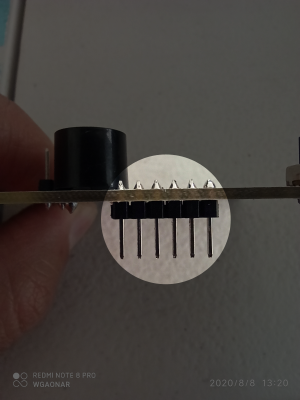
\includegraphics[width=0.9\columnwidth, height=1.2\columnwidth]{images/CPU/cpu_pines_botonera_1.png}
        \caption{Soldadura de los pines de conexión con la botonera.}
        \label{fig:cpu_pines_botonera_1}
    \end{subfigure}
    \caption{Soldadura del Buzzer.}
    \label{fig:cpu_buzzer}
\end{figure}

\subsection{Soldadura de los Pines para el Arduino y los pines de conexión a la Botonera}

\end{document}
